
\begin{frame}{Experimental setting}

    We run experiments over two distinct data sets of pairs $(p, v)$ with $p > 1,000,000$ and $2 \leq v \leq 8$.
    
    \begin{description}
        \item[all primes:] Primes where $v \mid p -1$.
        \item[$g = v$ primes:] Primes where $v \mid p -1$ and $v$ is a generator.
    \end{description}

    \pause
    \begin{table}[ht]
    \centering
    \begin{tabular}{lrr}
        \toprule
                                  & all  &  $g = v$  \\ \midrule
        \# pairs $(p, v)$      & 715  & 400       \\ 
        \# distinct $v$           & 7    & 4         \\
        \# distinct primes        & 322  & 323       \\ 
        \# $v$ per prime (average) & 4.51 & 1.48      \\ \bottomrule
    \end{tabular}
    \label{tab:experiments}
\end{table}
    
    \begin{itemize}
        \item We run experiments over \emph{all primes} for the smallest 10 generators.
        \item If $v\in\{4,5,8\}$ then $v\neq g$.
    \end{itemize}
\end{frame}


\begin{frame}{ElGamal Sequences $t$-tuple bound gap distribution}
    \begin{columns}
        \begin{column}{0.45\textwidth}
        \begin{center}
            Lower bound $\lambda(z)$ >0\\
            $t =2$ and $12\%$ outliers.
        \end{center}
            \begin{figure}
                \centering
                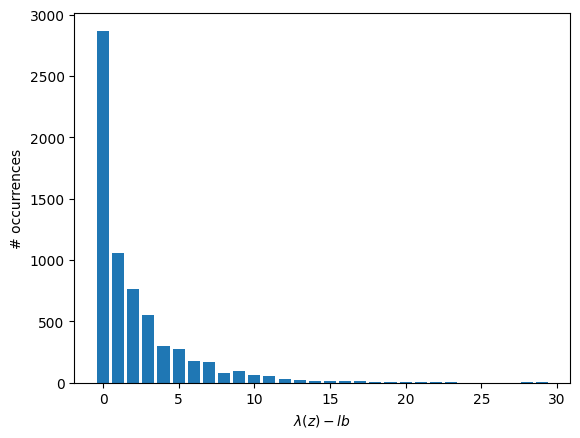
\includegraphics[width=\textwidth]{figures/LB0t2with012outliers.png}
            \end{figure}
        \end{column}
        \begin{column}{0.45\textwidth}
        \begin{center}
            Upper bound \\
            $t = 2$ and $5\%$ outliers
        \end{center}
            \begin{figure}
                \centering
                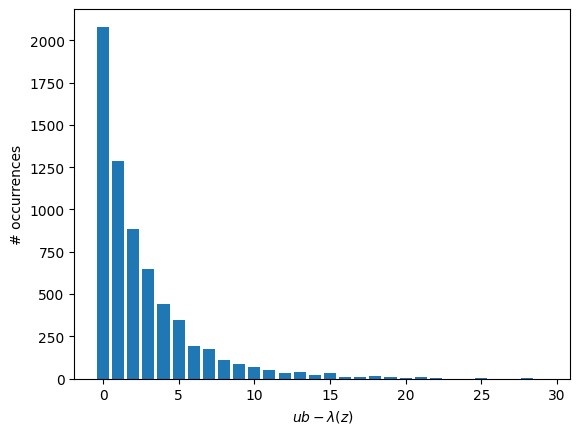
\includegraphics[width=\textwidth]{figures/UBt2with005outliers.png}
            \end{figure}
        \end{column}
    \end{columns}
    \begin{center}
                Distribution of gaps between $\lambda(z)$ and lower and upper bounds.
    \end{center}
\end{frame}


\begin{frame}{ElGamal Sequences $t$-tuple bound gap distribution}
    \begin{columns}
        \begin{column}{0.45\textwidth}
        \begin{center}
            Lower bound $\lambda(z)$ >0\\
            $t =7$ and $59.75\%$ outliers.
        \end{center}
            \begin{figure}
                \centering
                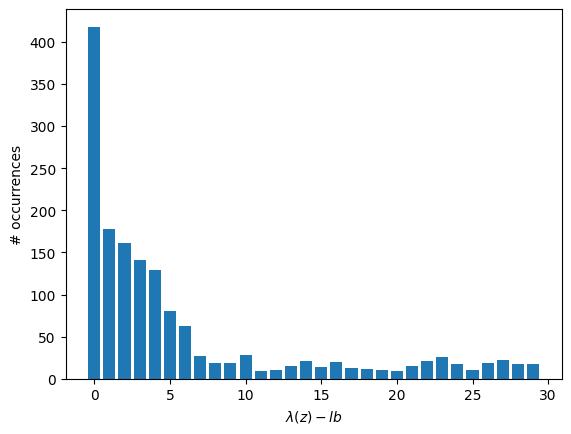
\includegraphics[width=\textwidth]{figures/LB0t7with5975outliers.png}
            \end{figure}
        \end{column}
        \begin{column}{0.45\textwidth}
        \begin{center}
            Upper bound \\
            $t = 7$ and $93.56\%$ outliers
        \end{center}
            \begin{figure}
                \centering
                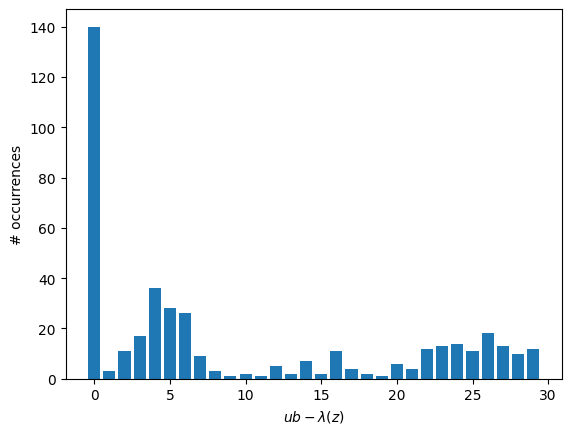
\includegraphics[width=\textwidth]{figures/UBt7with9356outliers.png}
            \end{figure}
        \end{column}
    \end{columns}
    \begin{center}
                Distribution of gaps between $\lambda(z)$ and lower and upper bounds.
    \end{center}
\end{frame}

\begin{frame}{ElGamal Sequences $t$-tuple bound accuracy}
    \begin{columns}
        \begin{column}{0.45\textwidth}
        \begin{center}
            Lower bound
        \end{center}
            \begin{figure}
                \centering
                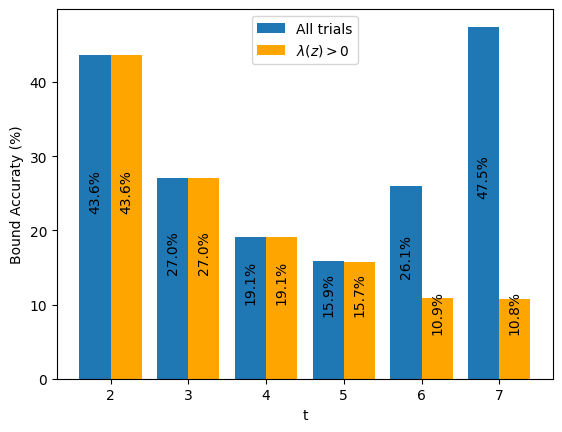
\includegraphics[width=\textwidth]{figures/TuplesLowerBoundAccuracy.png}
            \end{figure}
        \end{column}
        \begin{column}{0.45\textwidth}
        \begin{center}
            Upper bound 
        \end{center}
            \begin{figure}
                \centering
                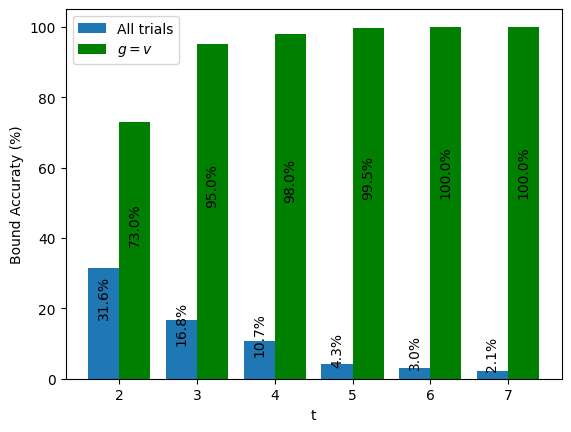
\includegraphics[width=\textwidth]{figures/TuplesUpperBoundAccuracy.png}
            \end{figure}
        \end{column}
    \end{columns}
    \begin{center}
                Percentage of trials with $z\in\mathbb{Z}_v^t$ s.t. $\lambda(z)$ matches lower and upper bounds.
    \end{center}
\end{frame}


\begin{frame}{ElGamal Sequences run bound accuracy}
    \begin{columns}
        \begin{column}{0.45\textwidth}
        \begin{center}
            Lower bound
        \end{center}
            \begin{figure}
                \centering
                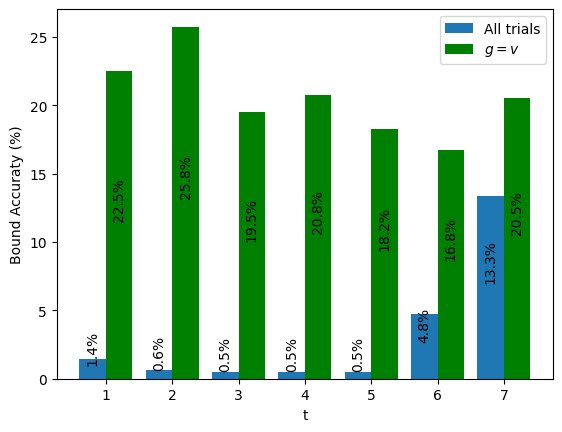
\includegraphics[width=\textwidth]{figures/RunsLowerBoundAccuracygisv.png}
            \end{figure}
        \end{column}
        \begin{column}{0.45\textwidth}
        \begin{center}
            Upper bound 
        \end{center}
            \begin{figure}
                \centering
                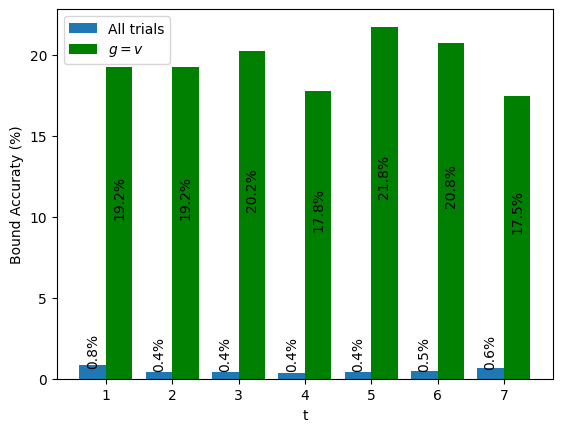
\includegraphics[width=\textwidth]{figures/RunsUpperBoundAccuracy.png}
            \end{figure}
        \end{column}
    \end{columns}
    \begin{center}
                Percentage of trials with $b\in\mathbb{Z}_v$ s.t. $\rho(b,t)$ matches lower and upper bounds.
    \end{center}
\end{frame}



\begin{frame}{ElGamal Sequences run ratio Experiment}
    \begin{columns}
        \begin{column}{0.45\textwidth}
        \begin{center}
            All primes.
        \end{center}
            \begin{figure}
                \centering
                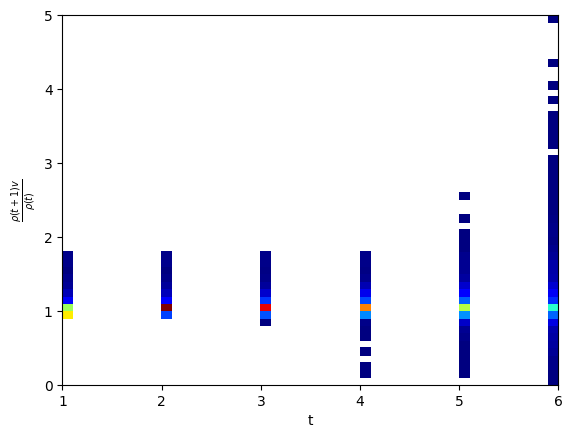
\includegraphics[width=\textwidth]{figures/AllDataNormalizedrunratio.png}
            \end{figure}
        \end{column}
        \begin{column}{0.45\textwidth}
        \begin{center}
            $g = v$ primes.
        \end{center}
            \begin{figure}
                \centering
                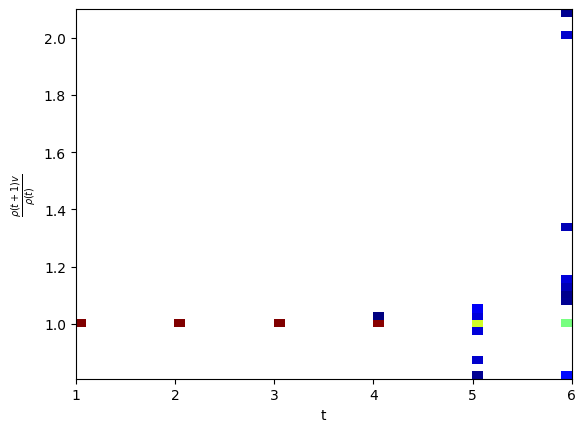
\includegraphics[width=\textwidth]{figures/AllDataAndvisGenNormalizedrunratio.png}
            \end{figure}
        \end{column}
    \end{columns}
    \begin{center}
                Distribution of $\rho(t+1)v/\rho(t)$ as a heat map with $2 \leq v \leq 8$
    \end{center}
\end{frame}

\begin{frame}{ElGamal Sequences run ratio Experiment}
    \begin{columns}
        \begin{column}{0.45\textwidth}
        \begin{center}
            All primes.
        \end{center}
            \begin{figure}
                \centering
                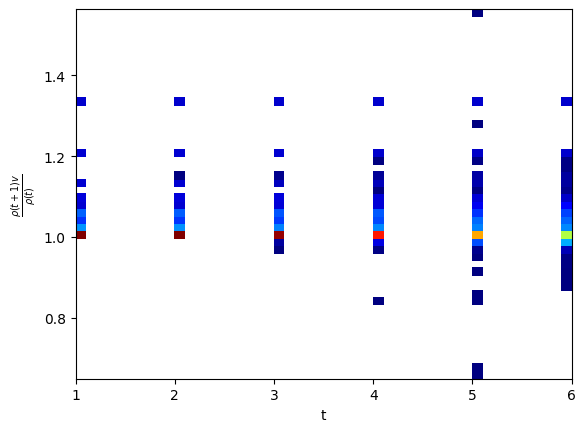
\includegraphics[width=\textwidth]{figures/v2Normalizedrunratio.png}
            \end{figure}
        \end{column}
        \begin{column}{0.45\textwidth}
        \begin{center}
            $g = v$ primes.
        \end{center}
            \begin{figure}
                \centering
                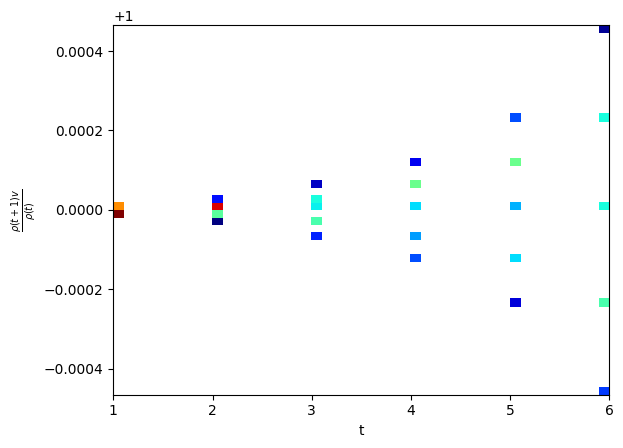
\includegraphics[width=\textwidth]{figures/v2AndvisGenNormalizedrunratio.png}
            \end{figure}
        \end{column}
    \end{columns}
    \begin{center}
                Distribution of $\rho(t+1)v/\rho(t)$ as a heat map with $v = 2$
    \end{center}
\end{frame}

%%% Local Variables:
%%% TeX-master: "../main.tex"
%%% End:
